\documentclass[border=3mm]{standalone}
\usepackage{tikz}
\usepackage[scaled=0.95]{helvet}
\renewcommand{\familydefault}{\sfdefault}
\begin{document}
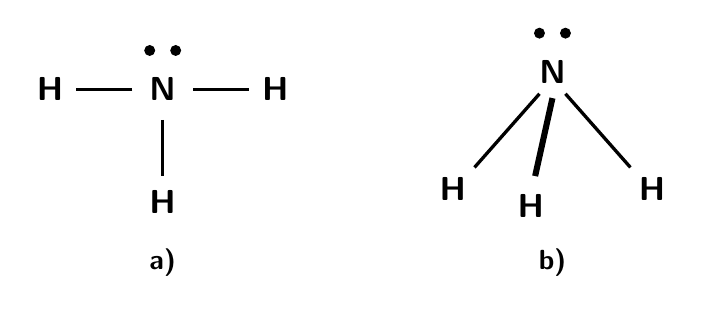
\begin{tikzpicture}[line width=1.1pt, scale=1.1]
  % Part a: Lewis structure
  \begin{scope}[shift={(0,0)}]
    \node at (0,0) {\large \textbf{N}};
    % lone pair on top
    \fill (-0.15, 0.45) circle (1.8pt);
    \fill (0.15, 0.45) circle (1.8pt);
    % bonds
    \draw (0, 0.25) -- (0, 0.25);
    \draw (-0.35, 0) -- (-1.0, 0);
    \node at (-1.3, 0) {\large \textbf{H}};
    
    \draw (0.35, 0) -- (1.0, 0);
    \node at (1.3, 0) {\large \textbf{H}};
    
    \draw (0, -0.35) -- (0, -1.0);
    \node at (0, -1.3) {\large \textbf{H}};
    
    \node at (0, -2.0) {\textbf{a)}};
  \end{scope}

  % Part b: Geometry (trigonal pyramidal)
  \begin{scope}[shift={(4.5,0)}]
    \node at (0,0.2) {\large \textbf{N}};
    % lone pair dots
    \fill (-0.15, 0.65) circle (1.8pt);
    \fill (0.15, 0.65) circle (1.8pt);
    
    % bonds
    \draw[line width=1.2pt] (-0.15, -0.05) -- (-0.9, -0.9);
    \node at (-1.15, -1.15) {\large \textbf{H}};
    
    \draw[line width=2.2pt] (0, -0.1) -- (-0.2, -1.0);
    \node at (-0.25, -1.35) {\large \textbf{H}};
    
    \draw[line width=1.2pt] (0.15, -0.05) -- (0.9, -0.9);
    \node at (1.15, -1.15) {\large \textbf{H}};
    
    \node at (0, -2.0) {\textbf{b)}};
  \end{scope}
\end{tikzpicture}
\end{document}
